\documentclass[a4paper,12pt]{article}

% Packages
\usepackage{graphicx}
\usepackage{amsmath}
\usepackage{hyperref}
\usepackage{xcolor}
\usepackage{listings}
\lstdefinestyle{mypython}{
    language=Python,
    basicstyle=\ttfamily\small,
    keywordstyle=\color{blue}\bfseries,
    stringstyle=\color{red},
    commentstyle=\color{green!50!black},
    breaklines=true,
    showstringspaces=false,
    frame=single,
    numbers=left,
    numberstyle=\tiny,
    numbersep=5pt,
}

% Title and Author
\title{Coin Classification Report}
\author{Tien Thang Dinh \\ Touch Sensing and Processing (WiSe24/25) \\ TU Dresden}
\date{\today}

\begin{document}

\maketitle

\section*{Introduction}
This report presents the results of a coin classification task using the given tactile images dataset. The goal of this project was to classify coins into six categories using a pre-trained Vision Transformer (ViT) from Hugging Face as a feature extractor and a custom classifier head. The dataset was split into training (80\%), validation (10\%), and test (10\%) subsets.

\section*{Methodology}
The model used in this project was the Vision Transformer (ViT), pre-trained on ImageNet ("google/vit-base-patch16-224"), \href{https://huggingface.co/google/vit-base-patch16-224}{link to model }. The feature extraction layers were frozen, and only the classifier head was trained. The following steps were performed:
\begin{itemize}
    \item \textbf{Dataset Preparation:} Scikit-learn was used for splitting the dataset with the ratio 80/10/10. After that, PyTorch's \texttt{ImageFolder} and \texttt{DataLoader} were used to prepare the dataset, where all images were resized to $224 \times 224$, as required by the ViT model. No augmentation was used.
    
    \item \textbf{Define the Model:}
The Vision Transformer (ViT) was adapted with a custom classifier head as shown in the following Python snippet:
\begin{lstlisting}[style=mypython]
model_name = "google/vit-base-patch16-224"
model = ViTForImageClassification.from_pretrained(model_name)
model.classifier = nn.Linear(model.config.hidden_size, len(train_loader.dataset.classes))
\end{lstlisting}


    \item \textbf{Training Loop Setup:} The model was trained for 10 epochs using a learning rate of $5 \times 10^{-5}$ and a batch size of 32. At each training iteration, metrics such as training loss, training accuracy, validation loss, and validation accuracy were calculated and saved for the report.

    \item \textbf{Test Model on Test Dataset:} After the training finished, a classification test on the test dataset was run, producing a confusion matrix.
\end{itemize}

\section*{Results}
Figure~\ref{fig:loss} shows the training and validation loss over 10 epochs. It is evident that the loss decreases steadily during training, indicating that the model is learning effectively. Interestingly, the validation loss (orange) is slightly lower than the training loss (blue) throughout the training. This might indicate that the validation set is simpler than the training set.

\begin{figure}[h!]
    \centering
    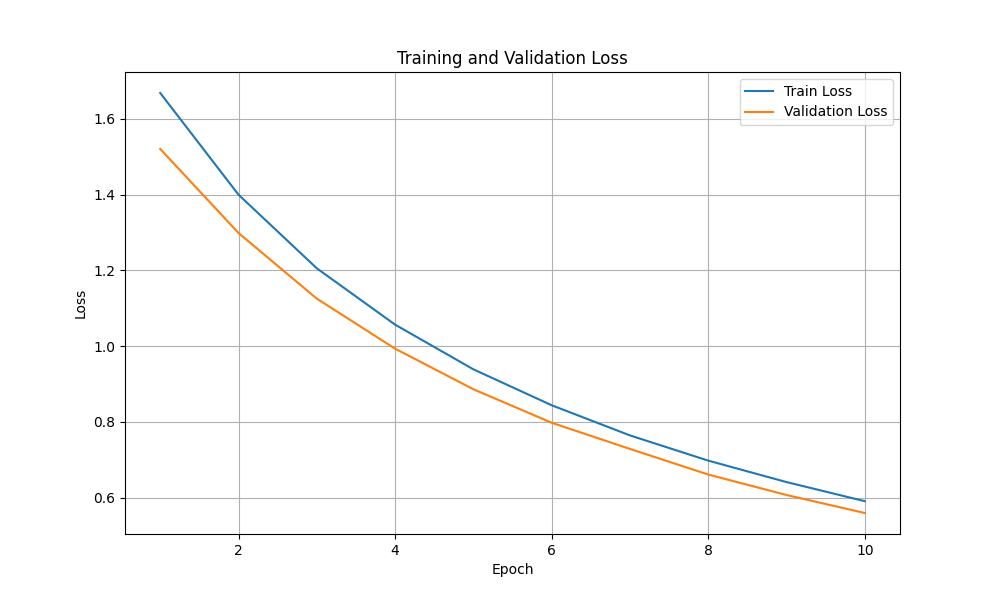
\includegraphics[width=1\textwidth]{train_val_loss_plot.png}
    \caption{Training and Validation Loss}
    \label{fig:loss}
\end{figure}

Figure~\ref{fig:accuracy} illustrates the training and validation accuracy, which improves significantly with each epoch. The final validation accuracy reached 94.05\%, demonstrating strong model performance. Similar to the loss trends, the validation accuracy (orange) is higher than the training accuracy (blue). This may really due to my assumption above that the validation set is actually simpler than training set. However the overal result indicates that the model is learning effectively.

\begin{figure}[h!]
    \centering
    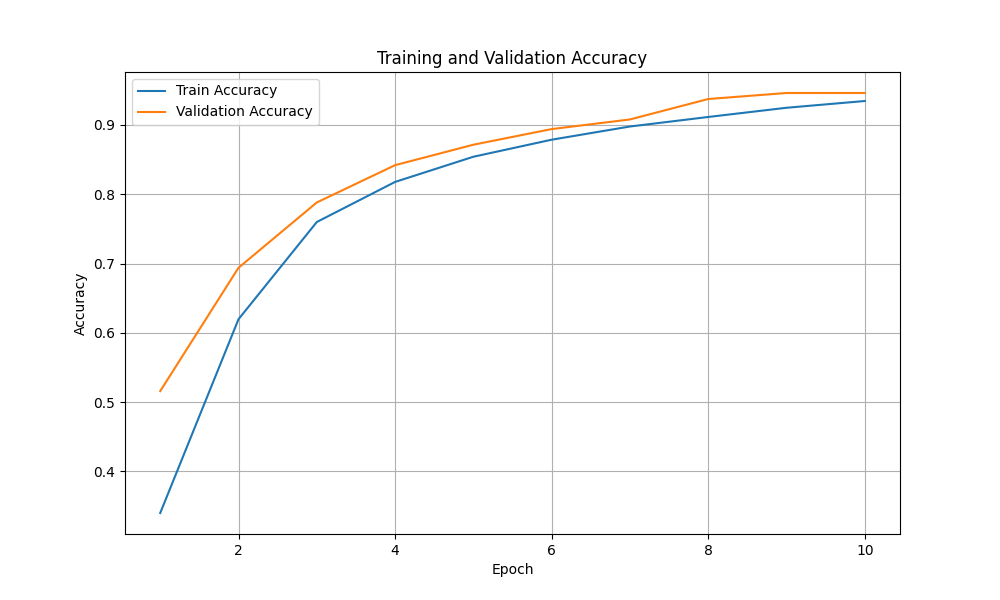
\includegraphics[width=1\textwidth]{train_val_acc_plot.png}
    \caption{Training and Validation Accuracy}
    \label{fig:accuracy}
\end{figure}

The confusion matrix for the test set is presented in Figure~\ref{fig:confusion}. It highlights the classification performance across all coin categories. The following things can be observed:

\begin{itemize}
    \item \textbf{High Accuracy:} Most classes have  high diagonal values, indicating strong classification performance.
    \item \textbf{Common missclassification:}
    \begin{itemize}
        \item The most confusion between \texttt{20cent} and \texttt{50cent}.
        \item This could be due to overlapping features between these classes. For example both \texttt{20cent} and \texttt{50cent} have \texttt{0} digit, as well as \texttt{2} and \texttt{5} both have a round path in its features.
    \end{itemize}
    \item \textbf{Best Performing Class:} The \texttt{1cent} class has the highest number of correctly classified examples (109) and is far better than the second best classes (87).
    \item \textbf{Challenging Classes:} The \texttt{20cent} performs the worst for the reason mention aboved.
\end{itemize}

\begin{figure}[h!]
    \centering
    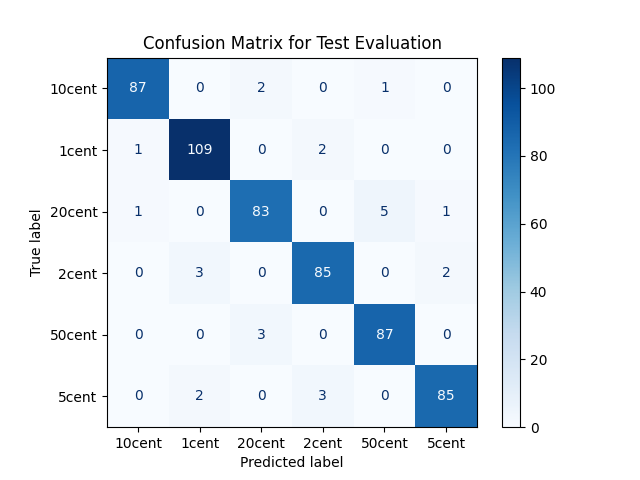
\includegraphics[width=0.8\textwidth]{confusion_matrix.png}
    \caption{Confusion Matrix for Test Set}
    \label{fig:confusion}
\end{figure}




\section*{Conclusion}
The Vision Transformer (ViT) model, fine-tuned with a custom classifier head, demonstrated effective coin classification with an accuracy of 95.37\% on the test set. The learning curves indicate steady improvement throughout training, and the confusion matrix highlights strong performance across all categories. 

This result suggests that the model is highly effective for tactile-based coin classification. Compared to a human using a single finger for similar tasks, this model not only achieves superior accuracy but also provides rapid inference that we as human might not be able to achieve. These findings open up exciting opportunities for practical applications in areas requiring accurate tactile-based classification where vision is not available.
\end{document}
